Adaptive changes are applied to software, when its environment changes. For instance, when a software system is installed on a computer, the installation can depend on configurations of the hardware, the software, and the device drivers for particular devices. If we move the software to a different computer that uses a different processor, installs a different operating system, and uses different drivers, the software will not execute. To overcome this problem and make the software executable again, we need adaptive changes to adjust the software to the new environment. 
Specifically, if the software system is written in a fully portable programming language (e.g., Go) that supports compilations for different platforms, we can recompile the source code of the software without manually applying any adaptive source code change for different operating systems and processors. For partially portable languages (e.g., C and C++) that contain some platform-specific library APIs, developers need to rewrite the part of the software implementation which depends on the platform-specific features. In extreme cases, e.g., when porting a Java desktop application to the iOS platform, developers need to rewrite everything from scratch, because both the programming language (i.e., Swift) and software libraries are totally different.  

In this section, we focus on three scenarios when adaptive changes are applied: cross-system software porting, cross-language software migration, and software library upgrade.

%\todo{Na, don't we need to describe changes coming from environment changes more broadly? I think it would make sense to include a category of feature addition. It seems to be the two categories of library update and cross-language transformation seem too narrow in its focus and not comprehensive enough to describe various kinds of software changes. Could we add a new category of platform update, changes to improve performance, etc? I hope you can update this overview paragraph and define the problems and challenges of adaptive changes more broadly and clearly.} 

\subsubsection{Cross-System Porting.} 
Software forking\textemdash creating a variant product by copying and modifying an existing product\textemdash is often considered an ad hoc, low cost alternative to principled product line development. To maintain such forked products, developers often need to port an existing feature or bug-fix from one product variant to another. 

\paragraph{\textbf{Empirical Studies on Cross-System Porting}}
Several studies analyzed the evolution of BSD product family. For example, Fischer et al.~analyzed change commit messages of the BSD family and found a decreasing trend of information flow between OpenBSD and other BSD projects~\cite{Fischer2005}. 
%Their analysis does not automatically identify similar code modifications made to different BSD projects. 
Yamamoto et al.~found that up to 40\% of lines of code were shared among NetBSD, OpenBSD, and FreeBSD~\cite{Yamamoto2005}. 
James et al.~showed the evidence of adopted code in device driver modules between Linux and FreeBSD~\cite{Cordy2011:largecloning}. 
%German et al.~also studied cross-project cloning in the BSD product family and analyzed copyright implications when code fragments transfer between different systems under different licenses. On the other hand, our study focuses on the characteristics of cross-system ported changes. 
Canfora et al.~investigated the social characteristics of contributors who made cross-system bug fixes between FreeBSD and OpenBSD~\cite{Canfora2011:bsdfork}. They used textual analysis of change commit logs and mailing list communication logs. They observed that 
%Their findings are aligned with our finding that 
contributors who port changes from other projects are highly active contributors. %Unlike Canfora et al., our study investigates all three projects (OpenBSD,  FreeBSD, and NetBSD), and automatically detects ported changes by determining similar edit content and edit operation sequences within release-level patches as opposed to the textual analysis of change commit messages only. Furthermore, our study extends Canfora et al.~by measuring the time taken to port changes, the percentage of files affected by porting, the workload distribution among the contributors who port patches from other projects, and the correlation between defects and ported changes vs. non-ported changes. 
Ozment et al.~investigated security vulnerabilities in the OpenBSD project to examine whether software security improves with age~\cite{Ozment2006}. %However, they did not investigate the extent and frequency of ported changes from other BSD projects. 
Ray et al.~\cite{Ray2012:FSE} comprehensively characterize the temporal, spatial, and developer dimensions of cross-system porting using the case study of BSD family. Their study found that maintaining forked projects involves significant effort of porting patches from other projects. Cross-system porting happens periodically and the porting rate does not necessarily decrease over time. A significant portion of active developers participate in porting changes from peer projects. Ported changes are less defect-prone than non-ported changes. 

\paragraph{\textbf{Cross-Platform Software Development}}
As shown in above-mentioned studies, when assigning different software development teams to independently work on separate source trees targeting different platforms, different teams maintain almost identical functionalities and incur a costly redundant developer effort. Some programming languages (e.g., 8th~\cite{8th}), software libraries (e.g., cairo~\cite{cairo}) and frameworks (e.g.,Ultimate++~\cite{ultimate}) have been built to facilitate cross-platform software development. With such tool support, developers only need to build software once, but get executable software for multiple platforms. 
%However, each of these tools focuses on specific programming task (e.g., GUI) or functionality (e.g., 2D graph drawing). 
In particular, HTML5 is designed to deliver almost everything customers may need without requiring additional software (e.g., browser plugins) to install~\cite{html5}. 
To simplify cross-platform mobile software development, some existing tools support developers to write code in HTML5 (e.g., Sencha~\cite{sencha}), or even automatically translate HTML5 implementation to Android or iOS native code (e.g., PhoneGap~\cite{phonegap}).

\subsubsection{Cross-language Migration.} 
When maintaining a legacy system that was written in an old programming language (e.g., Fortran) decades ago, programmers may migrate the system to a mainstream general-purpose language, such as Java, to facilitate the maintenance of existing codebase and to extend the system by leveraging new features of the popular language. 
%Different from the API adaptive changes mentioned above, such software translation requires of a significant amount of coding effort to rewrite the same application in a new programming language.
%\todo{Na, more techniques? I think this section is relatively weaker than others. I also do not think we can talk about TXL here, since we decided to talk about automated techniques separately.} 

\paragraph{\textbf{Cross-Language Program Translation}}
To translate code implementation from one language to another, most researchers built tools by hard coding the translation rules and implementing any missing equivalent functionality between languages~\cite{Yasumatsu:95,1192409:03,Sneed:2010}. SPiCE translates Smalltalk programs into a C environment by mapping the execution models of two languages. Specifically, Yasumatsu et al.~mapped compiled methods and contexts in Smalltalk to machine code and stack frames respectively, and implemented runtime replacement classes in correspondence with the Smalltalk execution model and runtime system~\cite{Yasumatsu:95}. Mossienko~\cite{1192409:03} and Sneed~\cite{Sneed:2010} automated COBOL-to-Java code migration by defining and implementing rules to generate Java classes, methods, and packages from COBOL programs. 
mppSMT is the most recent code translation tool, which automatically infers and applies Java-to-C\# migration rules using a phrase-based statistical machine translation approach~\cite{7372046}. It encodes both Java and C\# source files into sequences of syntactic symbols, called syntaxemes, and then relies on the syntaxemes to align code and to train a sequence-to-sequence translation model. %However, this approach depends on the highly similar program syntaxes between Java and C\#. It also requires tool builders to manually define rules to encode program syntactic components to syntaxemes. 


\paragraph{\textbf{Mining API Migration Rules}}
When migrating programs across languages, API usage conversion poses another challenge for developers who manually define program translation rules or reimplement software from scratch, because the diverse usage of API libraries induces an endless process of specifying API translation rules or identifying API mappings. Zhong et al.~\cite{zhong2010mining} and Nguyen et al.~\cite{nguyen2014statistical,Nguyen:2017:EAE} automatically mined API usage mappings between Java and C\#. Specifically, Zhong et al.~aligned the code in two versions based on similar names of classes and methods, and then constructed the API transformation graphs for each pair of aligned statements to identify API mappings~\cite{zhong2010mining}. StaMiner~\cite{nguyen2014statistical} mines API usage sequence mappings by conducting program dependency analysis~\cite{Muchnick:1998} and representing API usage as groums---a graph-based
model for representing object API usage~\cite{Nguyen09}. API2VEC mines API usage sequence mappings by converting API element sequences to vectors, and comparing cosine similarities between vectors~\cite{Nguyen:2017:EAE}. 

\subsubsection{Software Library Upgrade}

When building new software (e.g., a search engine), instead of coding everything from scratch, developers always extend existing frameworks or third-party libraries (e.g., Lucene~\cite{lucene}) by invoking the Application Programming Interfaces (APIs), to reuse the well implemented and fully tested functionality. However, as library developers release new versions of their software to fix existing bugs and include new features, client developers should also upgrade the libraries used in their projects to benefit from the newer versions. Ideally, the library APIs should be stable so that such software upgrades do not incur any program change in client applications. In reality, nevertheless, these APIs are susceptible to changes, requiring client developers to apply adaptive changes for the usage of new library versions. 


%Fig.~\ref{fig:releasenote} presents an exemplar library migration change 
\begin{comment}

\begin{figure}
\centering
\scalebox{0.4}{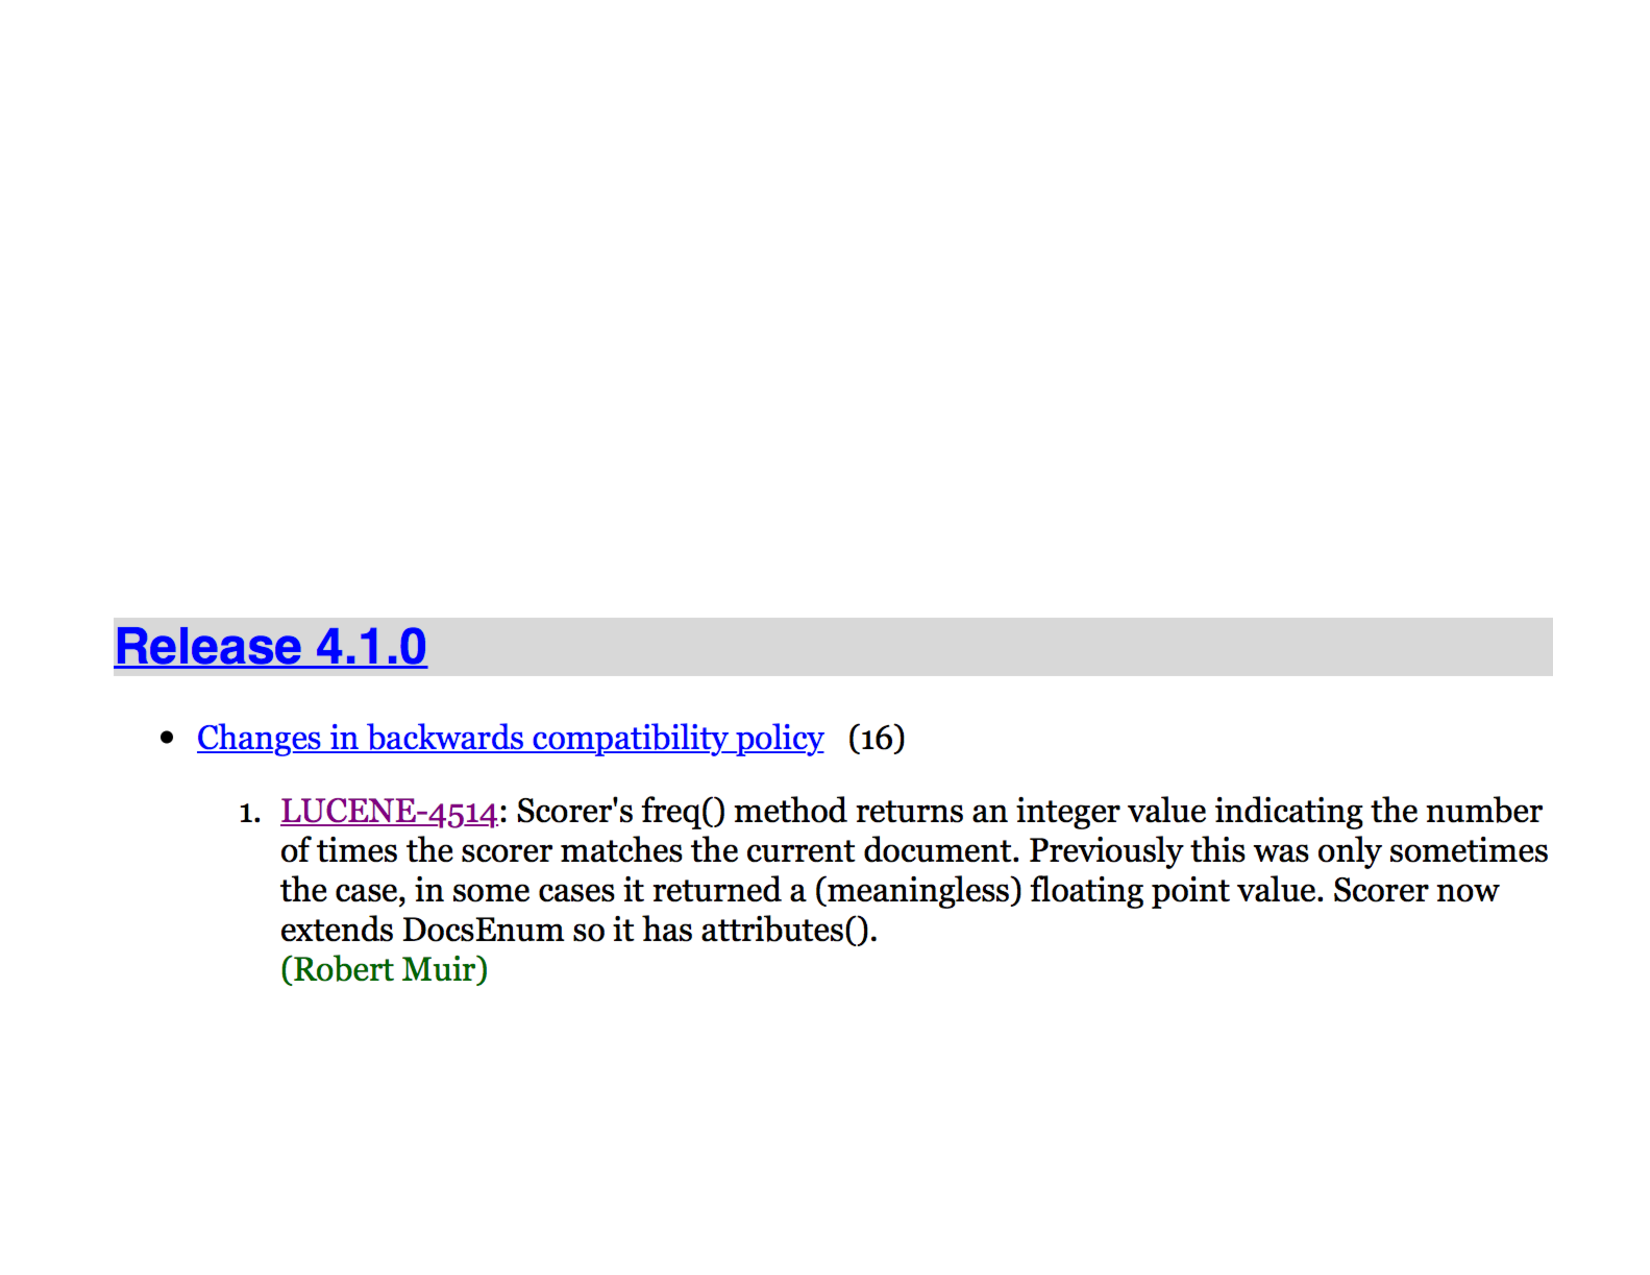
\includegraphics{images/releasenote.pdf}}
\caption{An excerpt of the Lucene change log for Release 4.1.0~\cite{releasenote}}
\label{fig:releasenote}
\end{figure}
\end{comment}

\paragraph{\textbf{Empirical Studides of API Evolution}}

Dig and Johnson \cite{Dig'05} manually investigated API changes using the change logs and release notes to study the types of library-side updates that break compatibility with existing client code, and discovered that 80\% of such changes are refactorings. Xing and Stroulia~\cite{Xing2006:apievol} used UMLDiff to study API evolution in several systems, and found that about 70\% of structural changes are refactorings. Kim et al.'s signature change pattern analysis \cite{Kim2006:apievol} categorizes API signature changes in terms of data-flow invariant. Yokomori et al.~\cite{Yokomori2009:apiimpact} investigated the impact of library evolution on client code applications using component ranking measurements. Padioleau et al.~\cite{Padioleau2006:collateral} found that API changes in the Linux kernel lead to subsequent changes on dependent drivers, and such collateral evolution could introduce bugs into previously mature code. 
McDonelle et al.~\cite{McDonnell2013:api} examine the relationship between API stability and the degree of adoption measured in propagation and lagging time in the Android Ecosystem. Hou and Yao study the Java API documentation and find that a stable architecture played an important role in supporting the smooth evolution of the AWT/Swing API~\cite{Hou2011:api}.  
In a large scale study of the Smalltalk development communities, Robbes et al.~found that only 14\% of deprecated methods produce non-trivial API change effects in at least one client-side project; however, these effects vary greatly in magnitude. On average, a single API deprecation resulted in 5 broken projects, while the largest caused 79 projects and 132 packages to break~\cite{robbes2012}.
Yau et al.~\cite{Yau1978} and Black~\cite{Black2001} investigate the ripple effects of evolving software, but these studies focus on a single system, as opposed to the impact of evolving APIs on clients.

\paragraph{\textbf{Automated Support for API Evolution and Client Adaptation}} 
There are several existing approaches to support client adaptations to cope with evolving libraries.  Chow and Notkin~\cite{Chow1996} proposed a method for changing client applications in response to library changes\textemdash a library maintainer annotates changed functions with rules that are used to generate tools that will update client applications. 

Henkel and Diwan's CatchUp~\cite{Henkel2005} records and stores refactorings in an XML file that can be replayed to update client code. However, its update support is limited to three refactorings: renaming operations (e.g.  types, methods, fields), moving operations (e.g. classes to different packages, static members), or change operations (e.g. types, signatures). The key idea of CatchUp, {\em record-and-replay}, assumes that the adaptation changes in client code are exact or similar to the changes in the library side. Thus, it works well for replaying rename or move refactorings or supporting API usage adaptations via inheritance. However, CatchUp cannot suggest programmers how to manipulate the context of API usages in client code such as the surrounding control structure or the ordering between method-calls.
% such as the example shown in Section~\ref{sec:empirical}. 
Furthermore, CatchUp requires that library and client application developers use the same development environment to record API-level refactorings, limiting its adoption in practice. Xing and Stroulia's Diff-CatchUp~\cite{Xing2007:diffcatchup} automatically recognizes API changes of the reused framework and suggests plausible replacements to the obsolete APIs based on working examples of the framework codebase.  Dig et al.'s MolhadoRef~\cite{Dig2007} uses recorded API-level refactorings to resolve merge conflicts that stem from refactorings; this technique can be used for adapting client applications in case of simple rename and move refactorings occurred in a library.  

SemDiff~\cite{Dagenais2008:RAC} mines API usage changes from other client code or the evolution of library itself. %similar to our work.  
%The key difference of {LibSync} from SemDiff is that with our work uses a graph-based representation to capture the context of an API usage, including the dependencies among method calls and with a surrounding control logic. In our work, an adaptation pattern is captured in term of a frequent set of graph editing operations that are common to multiple API usage skeletons before and after library migration. On the other hand, 
SemDiff defines an adaptation pattern as a frequent {\em replacement} of a method invocation. That is, if a method call to $A.m$ is changed to $B.n$ in several adaptations, $B.n$ is likely to be a correct replacement for the calls to $A.m$. As SemDiff models API usages in terms of method calls, it cannot support complex adaptations that involve multiple objects and method calls and that require the knowledge of the surrounding context of those calls. LibSync helps client applications migrate library API usages by learning migration patterns~\cite{Nguyen2010:GAA} with respect to a partial AST with containment and data dependences. Though it suggests what code locations to examine and shows example API updates, it is \emph{unable} to transform code.  Furthermore, its flexibility is limited by its inability to abstract variable, method, and type names.

A survey of techniques for easing API migration is found elsewhere~\cite{cossette2012}. Cossette and Walker found that, while most broken code may be mended using one or more of these techniques, each is ineffective when used in isolation~\cite{cossette2012}.  

\paragraph{\textbf{API Usage Specification Extraction}} 
There exist several approaches for extracting API usage specifications. The forms of recovered API usage specifications and patterns include finite state automaton~\cite{zeller07,doc2spec}, pairs of method calls~\cite{Livshits2005,williams-tse05}, partial orders of calls~\cite{mapo-fse07,taoxie-ase09}, and Computation Tree Logic formulas~\cite{zeller-ase09}. The API usage representations in those static approaches are still limited, for example, the patterns are without control structures and involve only individual objects belonging to one class. 
%Our graph-based API usage representation captures multi-object API usage patterns with control structures. 
In contrast to those static approaches, dynamic approaches recover the specifications by investigating the execution traces of programs~\cite{javert,perracotta,shoham-issta07,ramanathan-isce07,mike-ase09}.  These dynamic approaches require a huge amount of execution traces.  
%Our graph-based representation, iGROUM, captures API usage patterns with control and data dependencies among method calls, and surrounding control logic such as \codefont{while} loop and \codefont{if} statement. 
%The API usage representations in this paper extend our prior work on GRouMiner~\cite{Nguyen09} to tailor the original multi-object usage representation in order to capture the relevant context surrounding the use of external APIs. In particular, iGROUM explicitly captures API types and methods that appear in action and data nodes, so that program slicing can isolate only a sub-graph that is relevant to the use of a particular library. We also created a new model called xGROUM to represent overriding and inheritance relationships between client methods and API methods. 

